\parx
Figure \ref{fig:cn_docs} shows the Docs window for accessing the different
guides about particular topics in programming. This is accessible for users as
help when debugging and understanding certain warnings or errors in their
visual code.

\begin{figure}[H]
	\centering
	\captionsetup{justification=centering}
	\captionsetup[figure]{list=yes}
	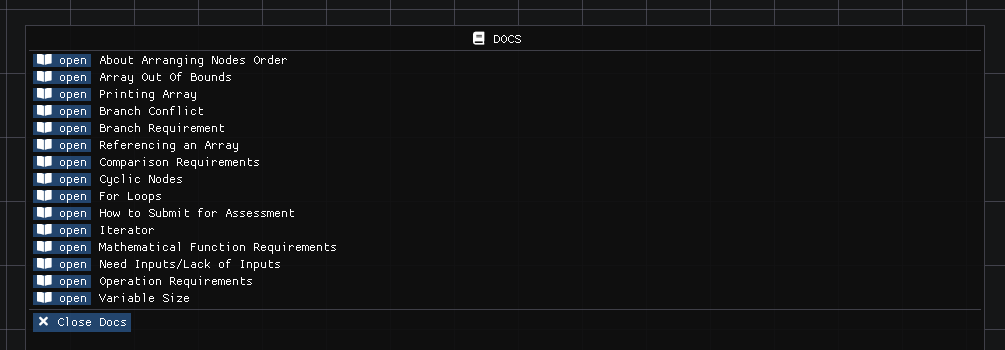
\includegraphics[width=\linewidth]{media/sc_docs.png}
	\caption[Screenshot of Docs in CodeNect]{Screenshot of Docs in CodeNect}
	\label{fig:cn_docs}
\end{figure}

\parx
Figure \ref{fig:cn_docs_sample} shows an example of a document in Docs window.
This document provides explanation, code example, and key points about
a particular topic.

\begin{figure}[H]
	\centering
	\captionsetup{justification=centering}
	\captionsetup[figure]{list=yes}
	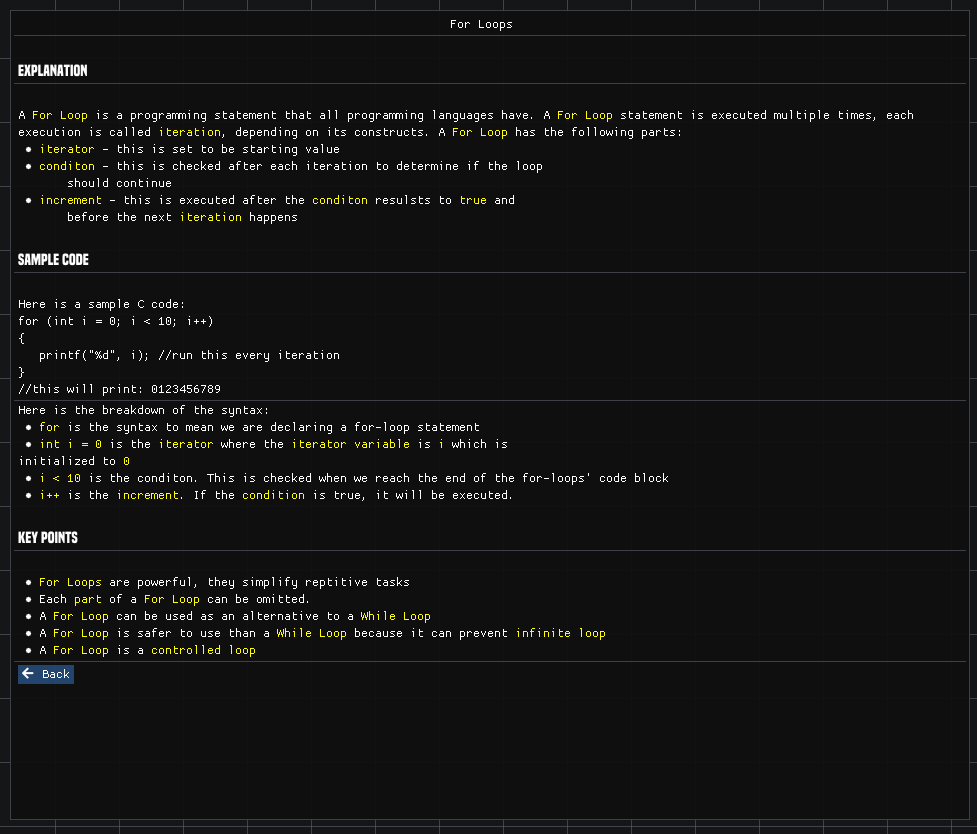
\includegraphics[width=\linewidth]{media/sc_docs_sample_for_loops.png}
	\caption[Screenshot of Sample Docs in CodeNect]{Screenshot of Sample Docs in CodeNect}
	\label{fig:cn_docs_sample}
\end{figure}
